\section{Simulator Instance}
Die \texttt{SimulatorInstance} unterscheidet sich bei jeder Anwendungsausprägung, aufgrund der verschiedenen Zusammensetzung von Softwarekomponenten, wie z.B. Netzwerkschnittstellen oder Tasks. Jedoch gibt es Komponenten, welche von mehreren der Anwendungen verwendet werden können. Im Folgenden wird die Grundstruktur der \texttt{SimulatorInstance} beschrieben, welche Komponenten diese verwenden kann und wie letztendlich die unterschiedlichen Instanzen aufgeteilt sind. 

Damit jede Simulatorinstanz von der \texttt{SimulatorMain} verwendet werden kann, implementieren diese ein gemeinsames Interface. Dieses heißt \texttt{ISimulator} und erweitert das Interface \texttt{ISimulatorViewAPI}. Die \texttt{ISimulatorViewAPI} definiert die Schnittstelle zwischen GUI-Komponente und der \texttt{SimulatorInstance}. Zum einen muss auf das Modell zugegriffen werden. Dieses wird über die Methode \texttt{getModel()} bereitgestellt. Des Weiteren wird noch ein ITargetUpdateListener benötigt, der vom ScenarioUpdater verwendet wird um Ziele über das Asterix-Interface zu versenden. Dieser wird mit der Methode \texttt{getTargetUpdater()} übergeben. Diese beiden Methoden bilden die \texttt{ISimulatorViewAPI}.

Der \texttt{AbstractSimulatorMain} benötigt den \texttt{ISimulator}, um diesen zu stoppen und um die GUI-Komponente die \texttt{ISimulatorViewAPI} übergeben. Deswegen ist die einzige Methode des Interfaces die \texttt{stop()}-Methode. Das Starten der \texttt{SimulatorInstance} wird vom \texttt{RestartService} übernommen und wird in Kapitel 4.2 gezeigt.

\subsection{Simulator Core}
Eine Komponente, die jede Instance enthält, ist das Datenmodell. Es wurde entschieden, dass das Modell des RadarSimulator mit einer kleinen Erweiterung, für alle drei Anwendungen genutzt wird. Dadurch kann nicht nur der Modell-Code wiederverwendet werden, sondern auch der Code zum Aufbauen und Bearbeiten des Modells bleibt identisch.

Da das Modell in jeder Anwendungsausprägung verwendet, ist es sinnvoll eine Klasse zu erstellen, die das Modell verwaltet und auf der die weiteren Simulator Instanzen aufbauen. Diese Klasse heißt \texttt{SimulatorCore}. Der \texttt{SimulatorCore} besitzt eine Methode zu Erstellen des Modells, welche nur von den erbenden Klassen aufgerufen werden kann. Auf Abbildung \ref{fig:SimulatorInstance} ist zu sehen, wie diese das \texttt{ISimulator-Interface} implementiert.


\begin{figure}[p]
    \centering
    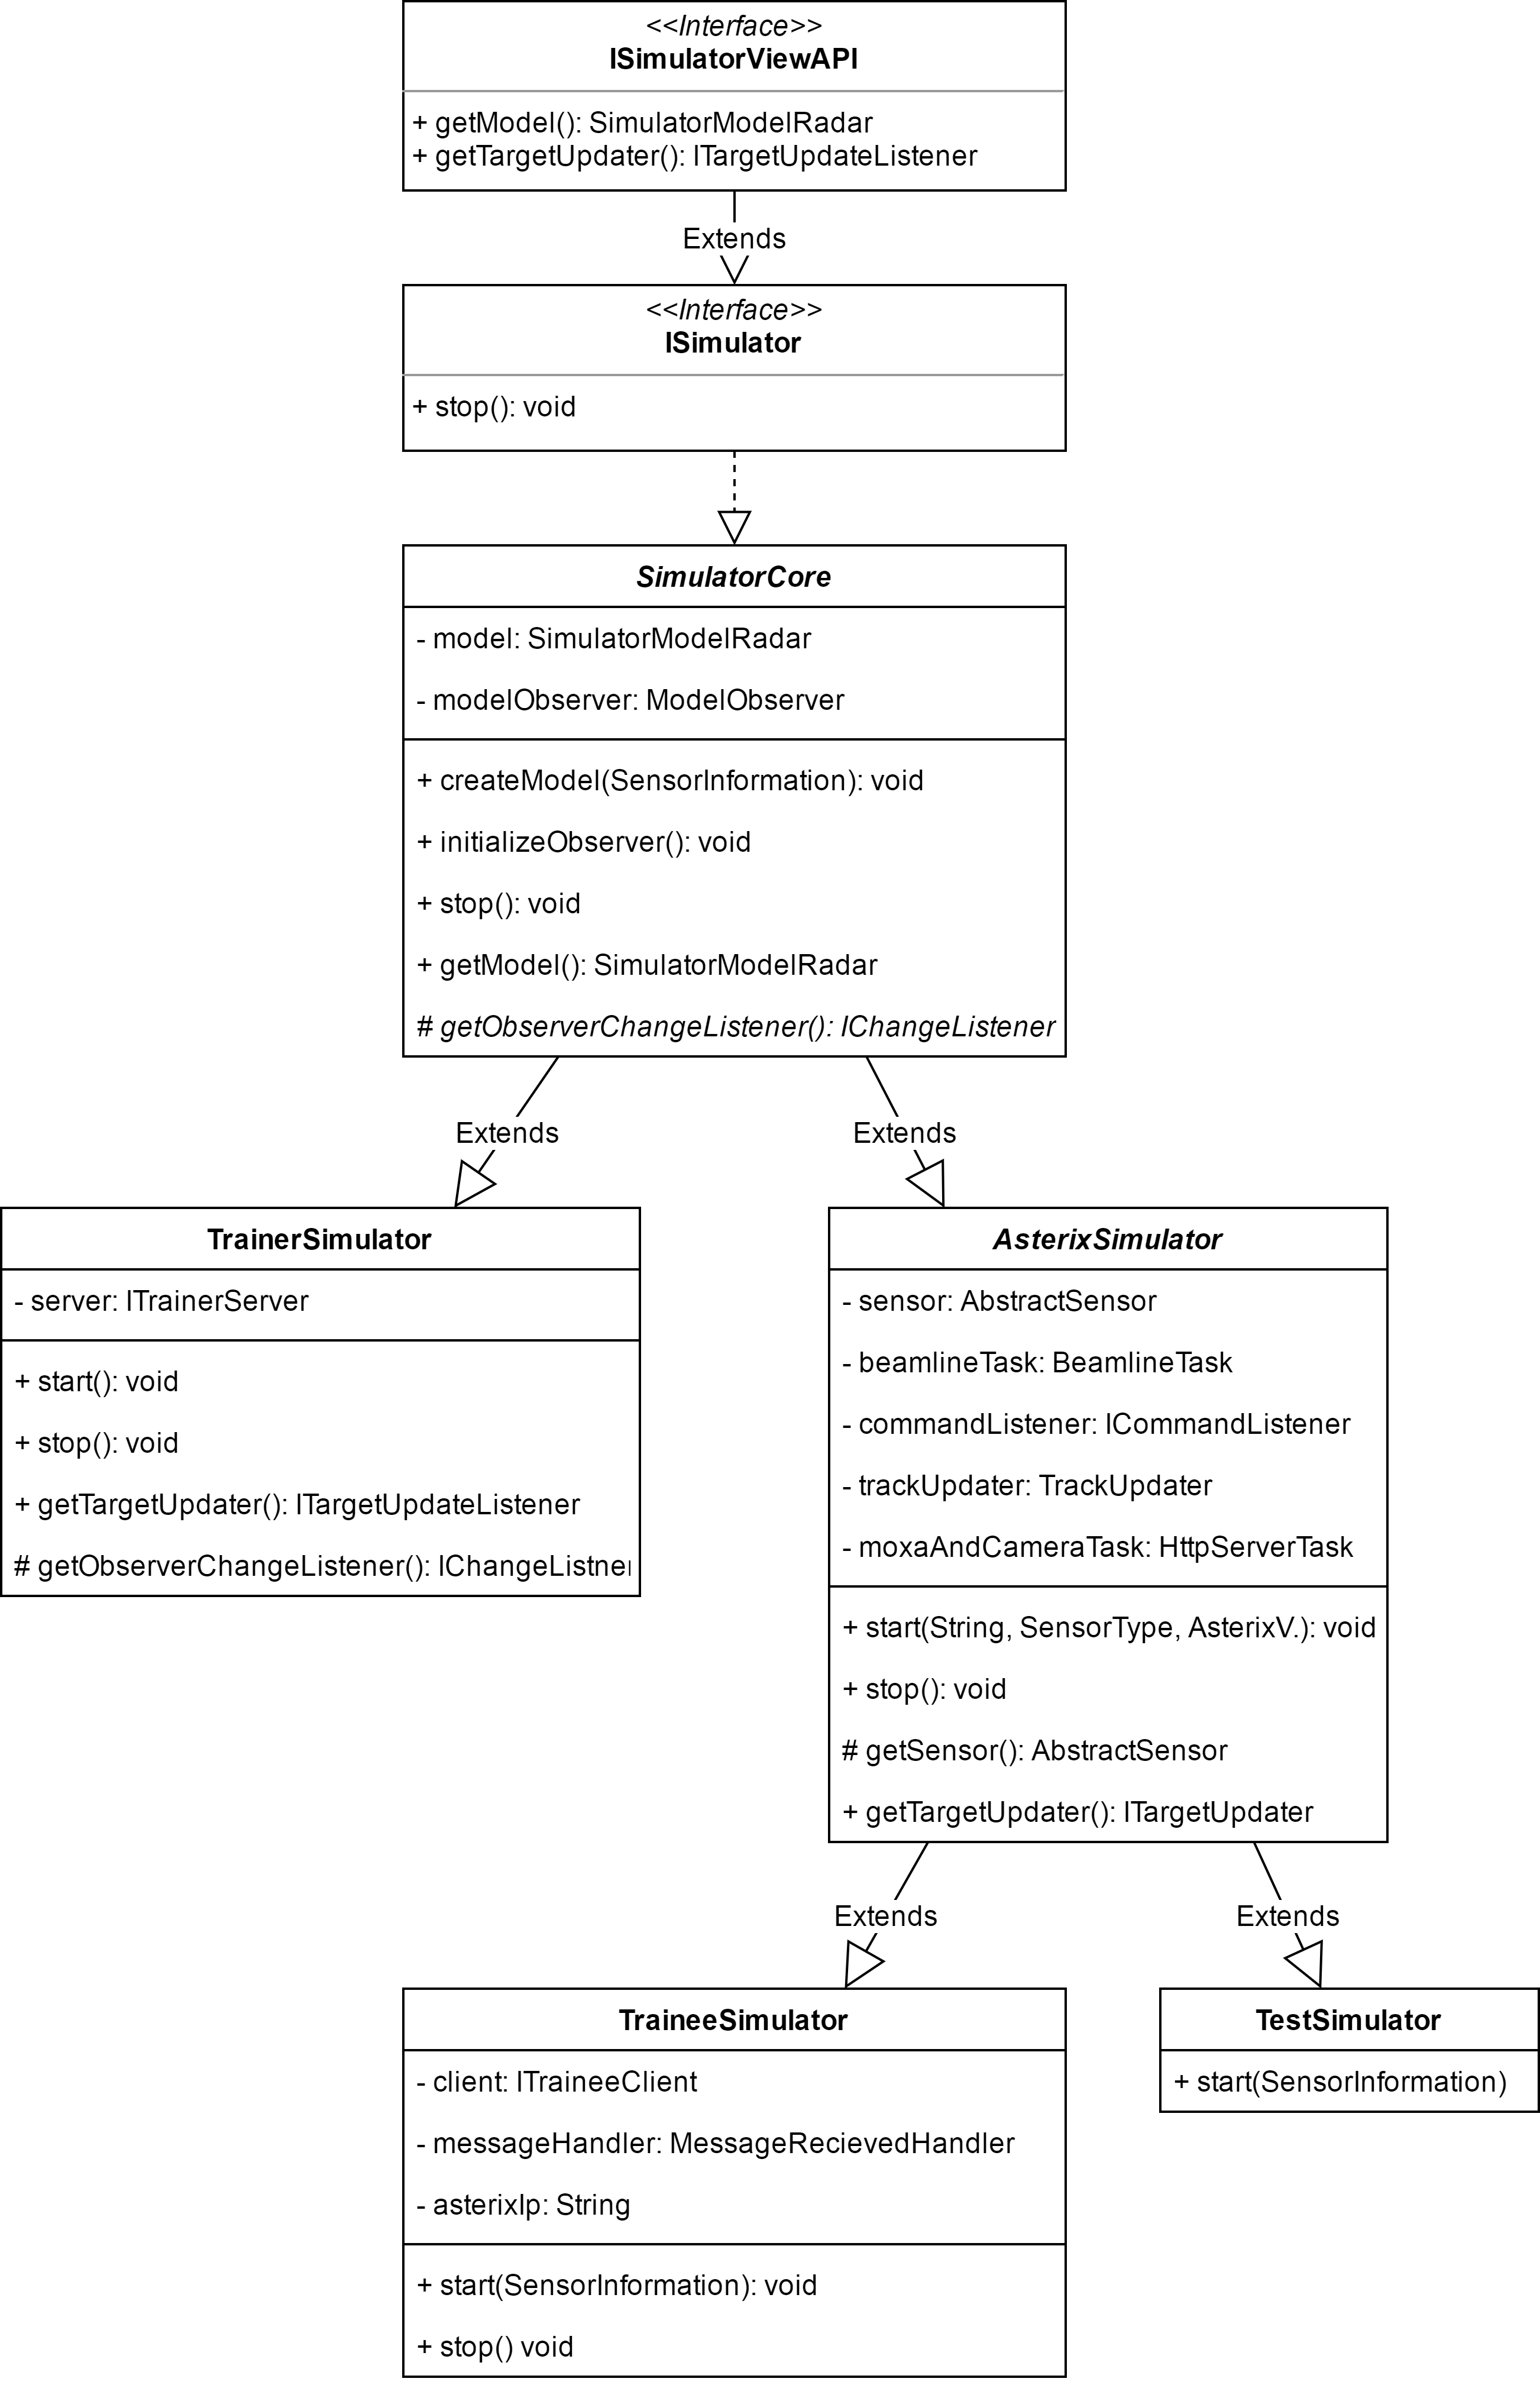
\includegraphics[width=0.85\textwidth]{content/assets/Kapitel4/SimulatorInstance.png}
    \caption{Die ausprägungen SimulatorInstance}
    \label{fig:SimulatorInstance}
\end{figure}

\subsection{Modell-Observer im SimulatorCore}
Eine weitere Funktion, welche im \texttt{SimulatorCore} implementiert wird, ist die des Modell-Observers. Wie in Kapitel 3.X gezeigt wurde, hat die Benutzeroberfläche des RadarSimulator zwei Abhängigkeiten. Das Model und den Sensor. In den neuen Anwendungen ist die GUI-Komponente nur noch vom Modell abhängig. 

\begin{figure}[ht]
    \centering
    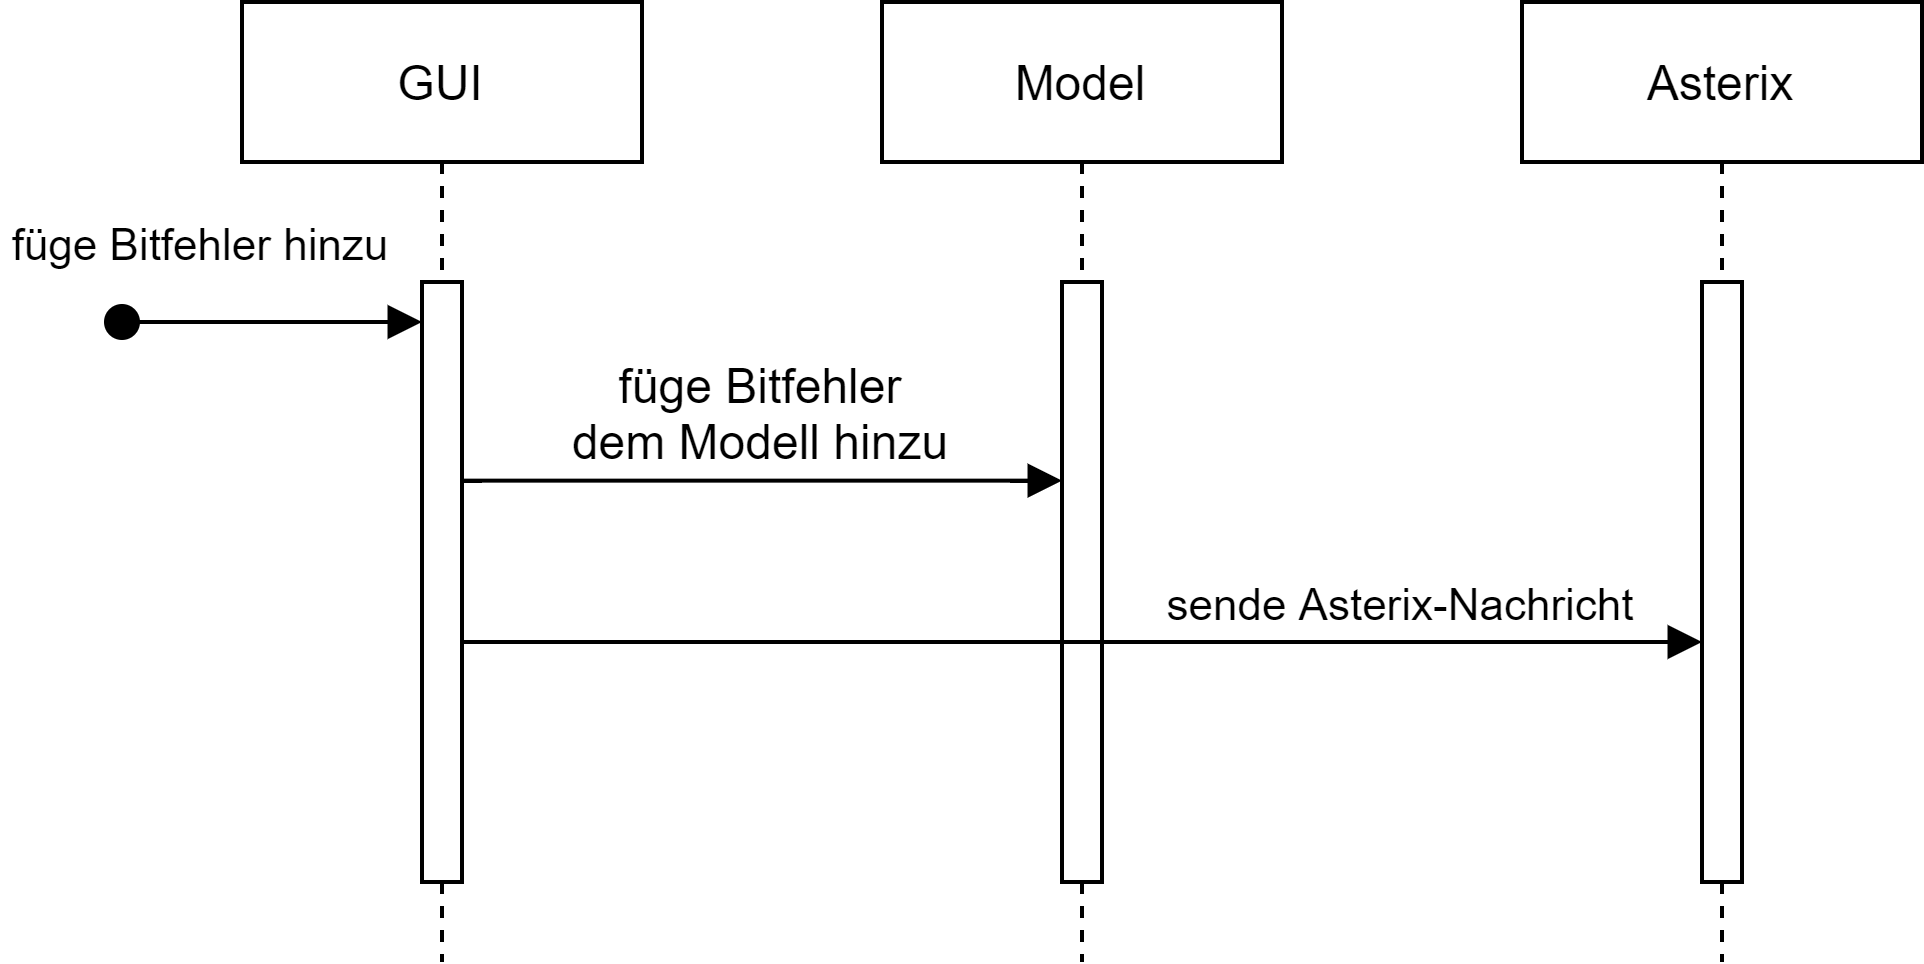
\includegraphics[width=0.7\textwidth]{content/assets/Kapitel4/AlterSimulator.png}
    \caption{Reaktion des alten RadarSimulator auf GUI-Änderung}
    \label{fig:SimulatorAlt}
\end{figure}

Um die Abhängigkeit der Benutzeroberfläche vom Sensor zu lösen, wird das Modell von so genannten Observern überwacht. Die Observer beobachten ein festgelegtes Objekt des Modells und führen bei einer Änderung dieses Objekts eine Methode aus. In diesen Methoden soll entweder der Sensor gesteuert oder die neue Netzwerkschnittstelle bedient werden. Diese Observerfunktion befindet sich ebenfalls im \texttt{SimulatorCore}. Im Sequenzdiagramm \ref{fig:SimulatorAlt} sieht man die Funktionsweise des alten Simulators. Im Sequenzdiagramm \ref{fig:SimulatorNew} die des neuen Simulators.

\begin{figure}[ht]
    \centering
    \includegraphics[width=0.85\textwidth]{content/assets/Kapitel4/NeuerTestSimulator.png}
    \caption{Reaktion der neuen Simulatoren auf GUI-Änderung}
    \label{fig:SimulatorNew}
\end{figure}


Zur besseren Übersicht des Codes, gibt es für verschiedene Bereiche des Modells eigene Observer. So gibt es z.B. für die Bitfehler einen \texttt
{BitModelObserver}. Jeder dieser Observer bekommt ein Interface übergeben, welches die verschiedenen Reaktionen des Observers, implementieren soll. Dieses Interface ist in Abbildung \ref{fig:SimulatorNew} als ModelChangeHandler zu erkennen. Um das an einem Beispiel zu verdeutlichen, wird der \texttt{BitModelObserver} des TrainerSimulator betrachtet. 

\begin{figure}[ht]
    \centering
    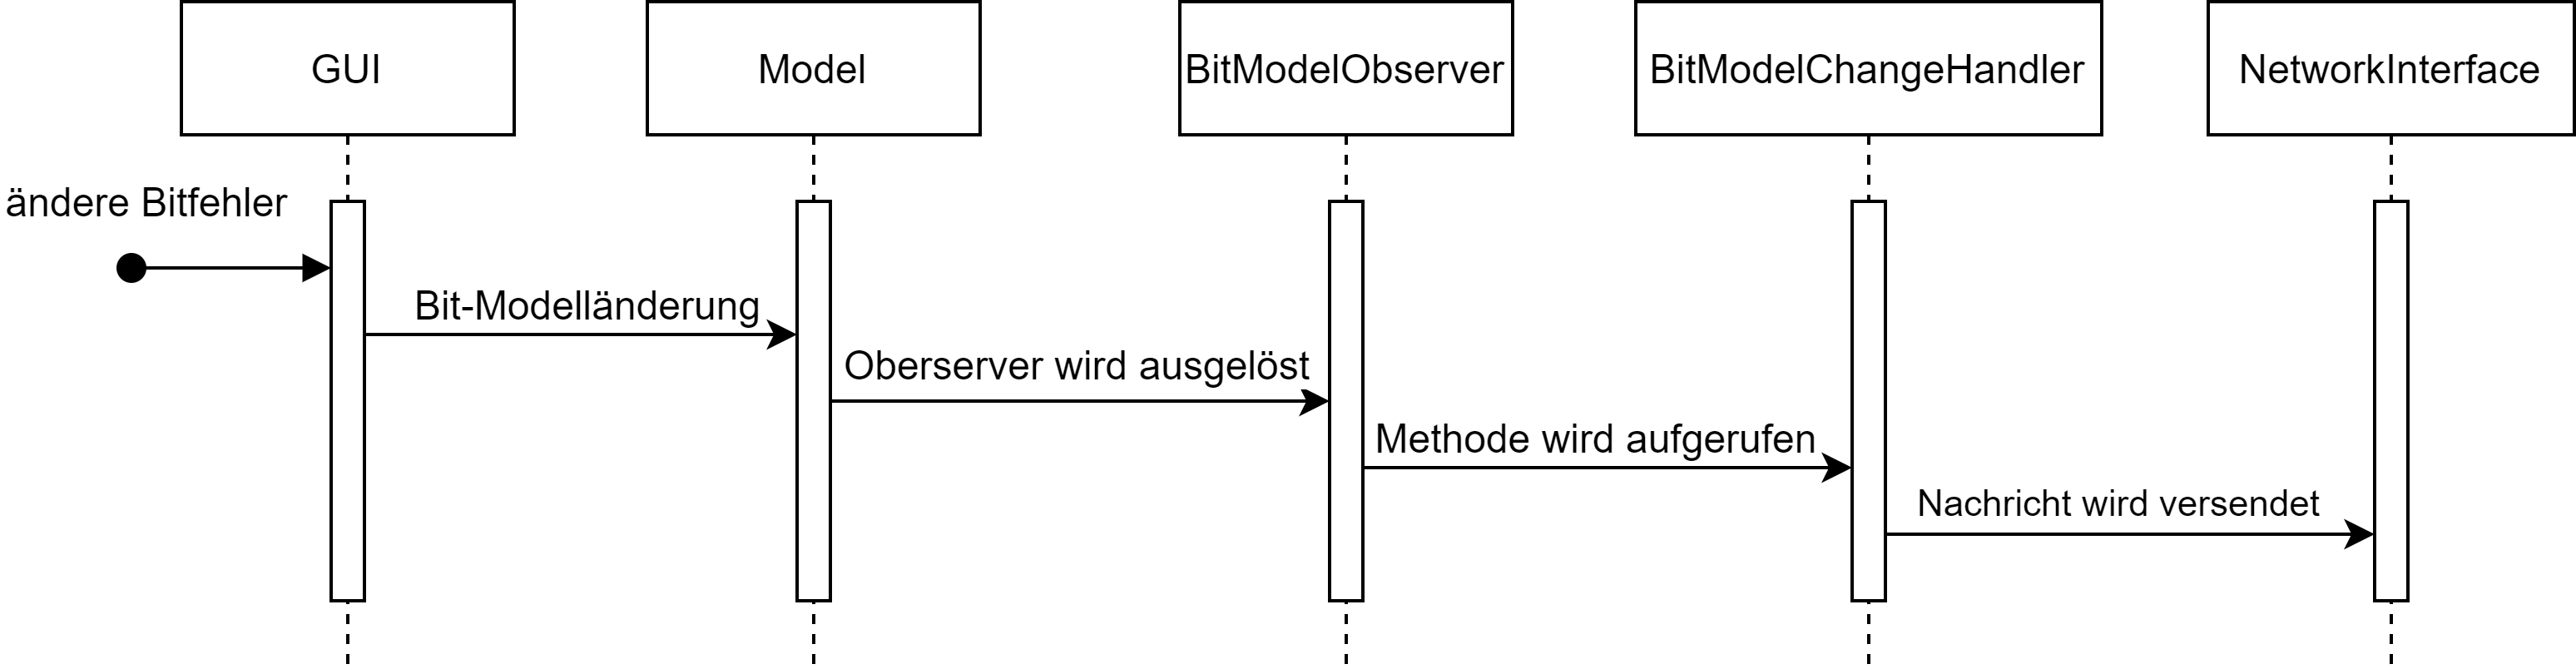
\includegraphics[width=1\textwidth]{content/assets/Kapitel4/BitChangeBeispiel.png}
    \caption{Reaktion des TrainerSimulator auf Bitänderung}
    \label{fig:TrainerNewBit}
\end{figure}

\sloppy
Der \texttt{BitModelObserver} beobachtet die \texttt{DefectReports} Liste im Modell. Mögliche Änderungen, die den Observer notifizieren sind das Hinzufügen, Ändern oder das Entfernen eines BitDefects. Damit auf diese Änderungen reagiert werden kann, wird ein Interface zur Verfügung gestellt. Dieses Interface heißt in diesem Fall \texttt{IBitModelChangeHandler}.
Die spezifischen Instancen müssen ein Objekt der Klasse \texttt{IBitModelChangeHandler} erstellen und übergeben. Dieses wird über die abstrakte Methode \texttt{getBitChangeHandler()} des \texttt{SimulatorCore} übergeben, welche jeder der erbenden Klassen implementieren muss. Der TrainerSimulator übergibt ein Objekt der Klasse \texttt{TrainerBitChangeHandler}, welches Nachrichten über den Server versendet.

\subsection{TrainerSimulator}
Wie man auf Abbildung \ref{fig:SimulatorInstance} erkennen kann erbt sie Instance-Klasse des Trainersimulators direkt vom \texttt{SimulatorCore} und heißt \texttt{TrainerSimulator}. Dieser erweitert den \texttt{SimulatorCore} um einen \texttt{TrainerServer}. Dieser ist dafür zuständig, dass veränderte Daten im Modell an die Trainees versendet werden.

Jeder der verwendbaren SimulatorInstancen besitzt eine Methode namens \texttt{start}, um die Instanz zu starten. Als Parameter der start-Methode werden Verbindungsdaten und Sensorinformationen eingeben. Beim Aufruf der \texttt{start()} Methode wird zu Beginn das Modell, abhängig von den Sensorinformationen erstellt und gefüllt. Daraufhin wird ein \texttt{ITrainerServer}-Objekt erzeugt und gestartet. Nachdem Modell und Server initialisiert sind, werden die Modellobserver erstellt, welche die \texttt{TrainerModelChangeListener} übergeben bekommen. Die \texttt{TrainerModelChangeListener} verwenden den \texttt{TrainerServer}, um Nachrichten an die Clients zu senden. Neben dem Observer wird noch ein lokaler Ordner erstellt, um Szenarien, die der Trainer im Benutzerinterface erstellt hat, zu speichern.

Das\texttt{ISimulatorViewAPI}-Interface des \texttt{TrainerSimulators} benötigt noch eine  implementierte {getTargetUpdater()}-Methode, welche dafür zuständig ist, dass TargetSimulations, die vom \texttt{ScenarioUpdater} kommen, versendet werden können. Auf Abbildung \ref{fig:TrainerTargetSimulation} ist zu erkennen wie der \texttt{ScenarioUpdater}, dem ihm übergebenen \texttt{ITargetUpdaterListener} aktiviert. In diesem Fall ist das der \texttt{TargetSimulationNetworkUpdater}, welcher Nachrichten über den \texttt{ITrainerServer} sendet.

\begin{figure}[ht]
    \centering
    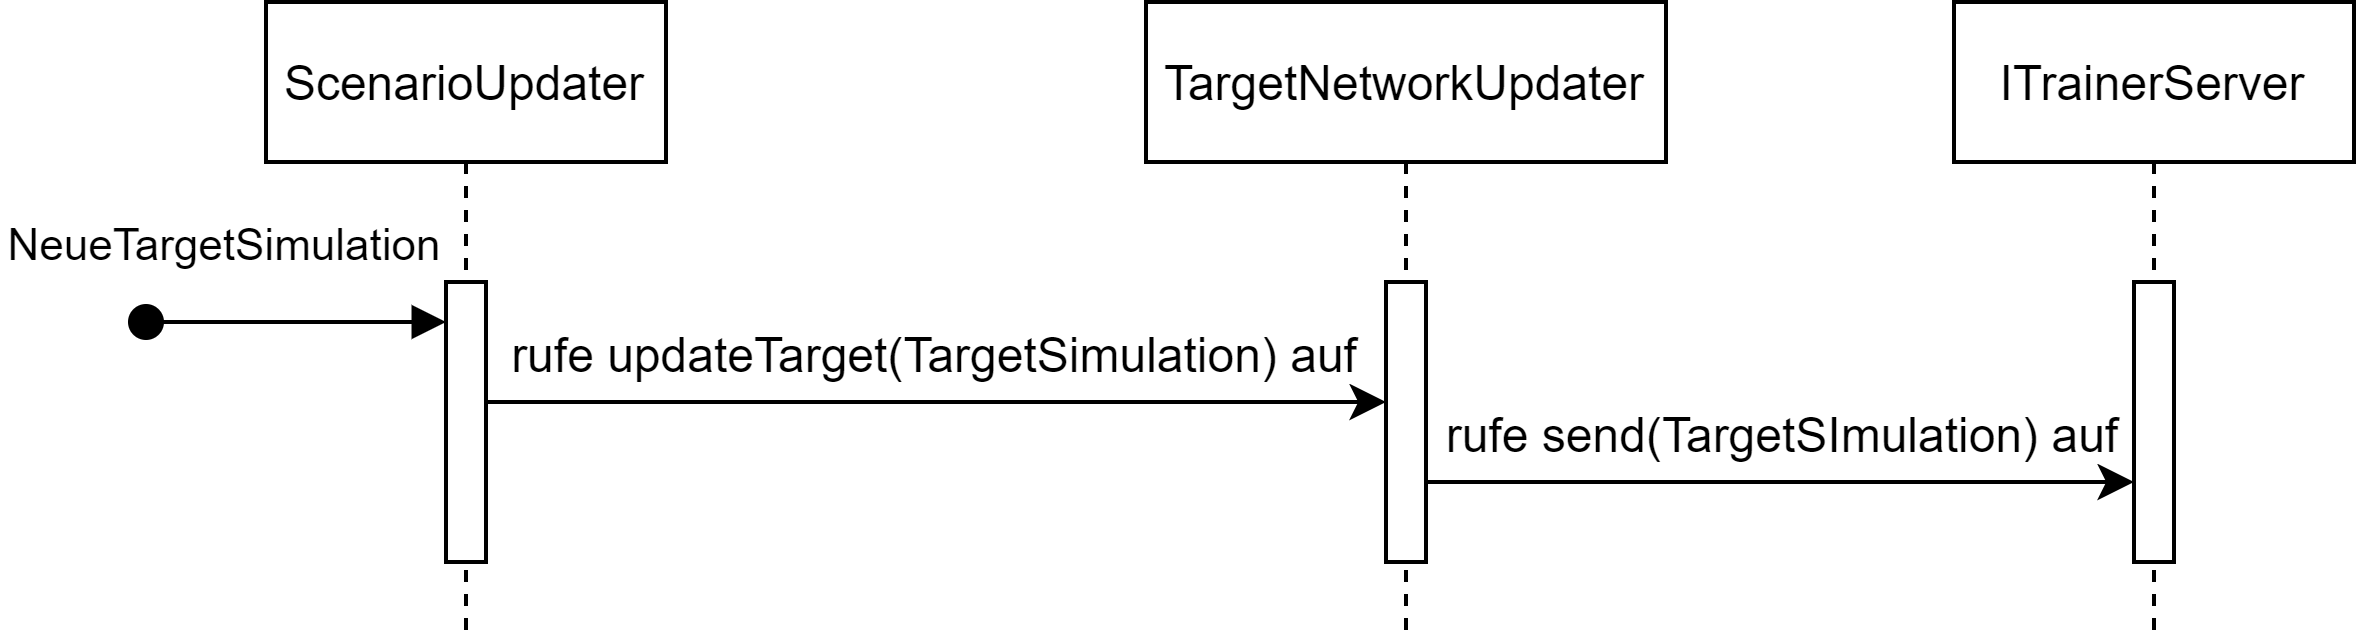
\includegraphics[width=0.9\textwidth]{content/assets/Kapitel4/TargetSimulationNetwork.png}
    \caption{TrainerSimulator sendet TargetSimulation}
    \label{fig:TrainerTargetSimulation}
\end{figure}

\subsection{AsterixSimulator}
Der Trainee-, sowie der Testsimulator bauen eine Verbindung zur Venus auf. Deshalb benötigen deren Instanzen einene \texttt{AbstractSensor}, welcher ein Asterix-Interface zur Verfügung stellt. Außerdem verwenden beide Anwendungen einen \texttt{TrackUpdater}, einen \texttt{BeamlineTask} und einen \texttt{moxaAndCameraServerTask}, die den \texttt{AbstractSensor} steuern un das Verhalten eines realen Sensors simulieren. Neben dem \texttt{AbstractSensor} brauchen beide auch einen entsprechenden \texttt{CommandListener}, der auf eingehende Kommandos des Asterix-Interfaces reagiert und passende Modelländerungen vornimmt.

Damit diese Funktionen nicht für die \texttt{TraineeInstance} und die \texttt{TestInstance} einzeln definiert werden müssen, wird die Komponente \texttt{AsterixSimulator} erstellt. Diese übernimmt die aufgezählten Funktionen und erbt von der Klasse \texttt{SimulatorCore}. Somit enthält diese auch das Model, Observer und den Code zur Unterstützung.

Wie der \texttt{TrainerSimulator}, muss auch ein \texttt{AsterixSimulator} auf Modelländerungen reagieren. Modeländerungen des Test- und des \texttt{TraineeSimulators} werden gleich gehandhabt. Auf eine Modelländerung folgt eine Asterix-Nachricht. Dabei gibt es ein paar Ausnahmen, bei denen keine Nachricht versendet werden muss. Diese werden durch den Modell-Observer geregelt, indem dieser nur relevante Modelldaten observiert. Die Objekt, welches die Modelländerungen handhaben, müssen das \texttt{IModelChangeListener}-Interface implementieren und werden über die abstrakten Klassen \texttt{getObserverChangeListener()} übergeben. Im Sequenzdiagramm \ref{fig:AsterixSimulator} wird dargestellt, wie der Ablauf nach einer Modelländerung ist. 

\begin{figure}[ht]
    \centering
    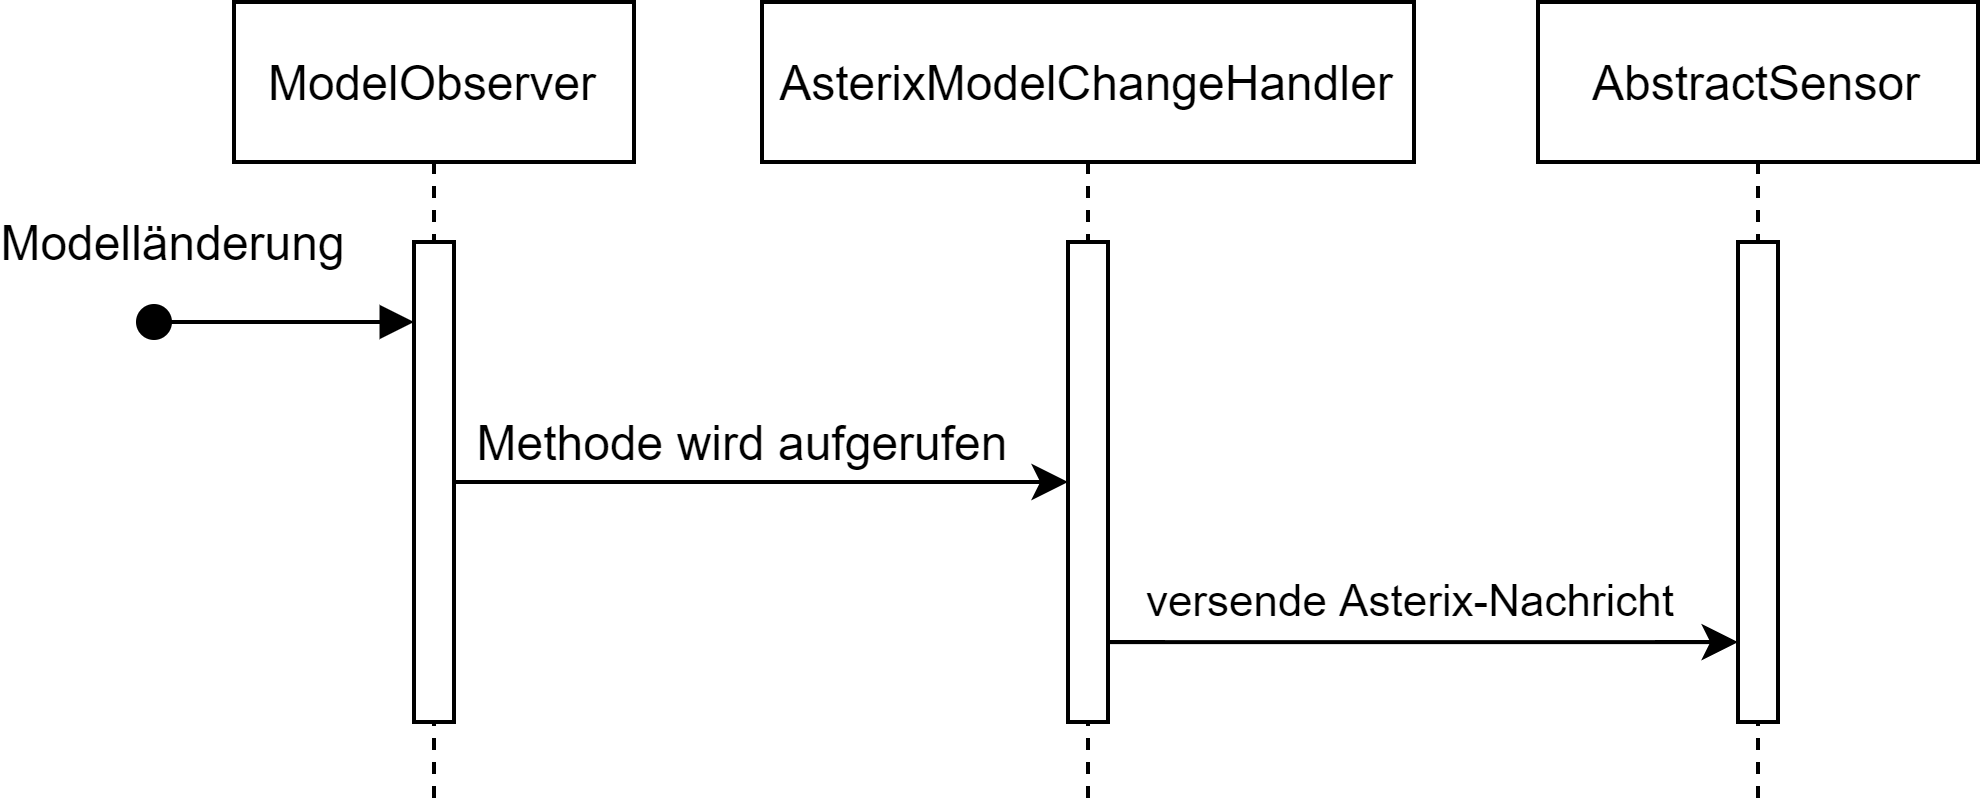
\includegraphics[width=0.9\textwidth]{content/assets/Kapitel4/AsterixSimulator.png}
    \caption{AsterixSimulator reagiert auf Modelländerung}
    \label{fig:AsterixSimulator}
\end{figure}

\subsection{TraineeSimulator}

Der \texttt{TraineeSimulator} erweitert den \texttt{AsterixSimulator}. Diese Instanz muss eine Verbindung zum \texttt{TrainerServer} aufbauen. Dafür verwendet der \texttt{TraineeSimulator} einen \texttt{TraineeClient}. Erst nachdem dies geschehen ist kann das Modell des Trainees geladen werden, da dieser den Sensortyp und die AsterixVersion vom Trainer übertragen bekommt.

Wenn der Server Daten an die verbundenen \texttt{TraineeClients} versendet, wird deren \texttt{MessageReceivedHandler} ausgelöst. Dies passiert über das Interface \texttt{IMessageRecievedListener}, welches die Methode \texttt{messageRecieved()} implementiert. Der \texttt{MessageReceivedHandler} entscheidet, wie mit den empfangenen Nachrichten umgegangen wird. Es gibt drei Arten von Nachrichten. Diese sind:

\begin{enumerate}
    \item Nachrichten, die \texttt{Sensorinformationen} beinhalten.
    \item Nachrichten, die das Modell updaten.
    \item Nachrichten, die \texttt{TargetSimulations} für den \texttt{TrackUpdater} beinhalten
\end{enumerate}

Nachrichten der 1. Art werden empfangen, wenn eine Verbindung zu einem Server aufgebaut wird. Daraufhin wird ein neues Modell und ein neuer \texttt{AbstractSensor} basierend auf den Informationen erstellt. Die Nachrichten 2. Art werden einfach dem Modell hinzugefügt und die der 3. Art dem \texttt{TrackUpdater}.

\subsection{TestSimulator}
Die Instance des \texttt{TestSimulators} baut auch auf dem \texttt{AsterixSimulator} auf. Die Klasse benötigt lediglich eine \texttt{start()}- Methode und muss einen Ordner erstellen, in dem Scenarios gespeichert werden. Dadurch funktioniert der \texttt{TestSimulator} wie der \texttt{RadarSimulator}.